\chapter{TP : Commande des moteurs avec Arduino}
\minitoc
\newpage

\section{Moteur à courant continu et module relais}
Dans un système robotique, les moteurs (à courant continu, servomoteurs ou pas à pas) sont les actionneurs les plus courants pour générer du mouvement. 
Étant donné que les sorties de la carte Arduino ne délivrent pas assez de puissance (maximum 40 mA sous 5V), nous utilisons des modules relais.
Ces derniers agissent comme des interrupteurs commandés, séparant le circuit de commande du circuit de puissance du moteur.

\paragraph{Exercice 1 : Commande d'un moteur dans les deux sens}
Dans cet exercice, nous utilisons deux relais pour créer un pont en H électromécanique.
Cela permet de contrôler le sens de rotation du moteur à courant continu en toute sécurité, sans risque de court-circuit.

\begin{figure}[H]
	\centering
	\begin{minipage}{0.48\textwidth}
		\centering
		 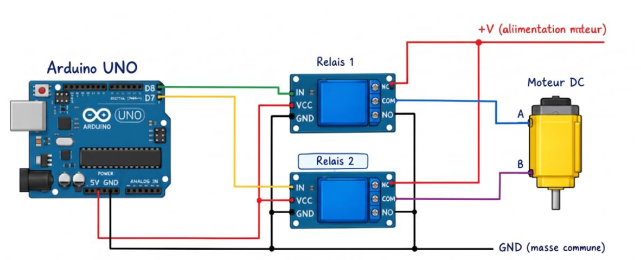
\includegraphics[width=\linewidth]{Image/4.Schema_Relais}
		\caption{Schéma de la commande avec deux relais}
		\label{fig:schema_relais}
	\end{minipage}\hfill
	\begin{minipage}{0.48\textwidth}
		\centering
		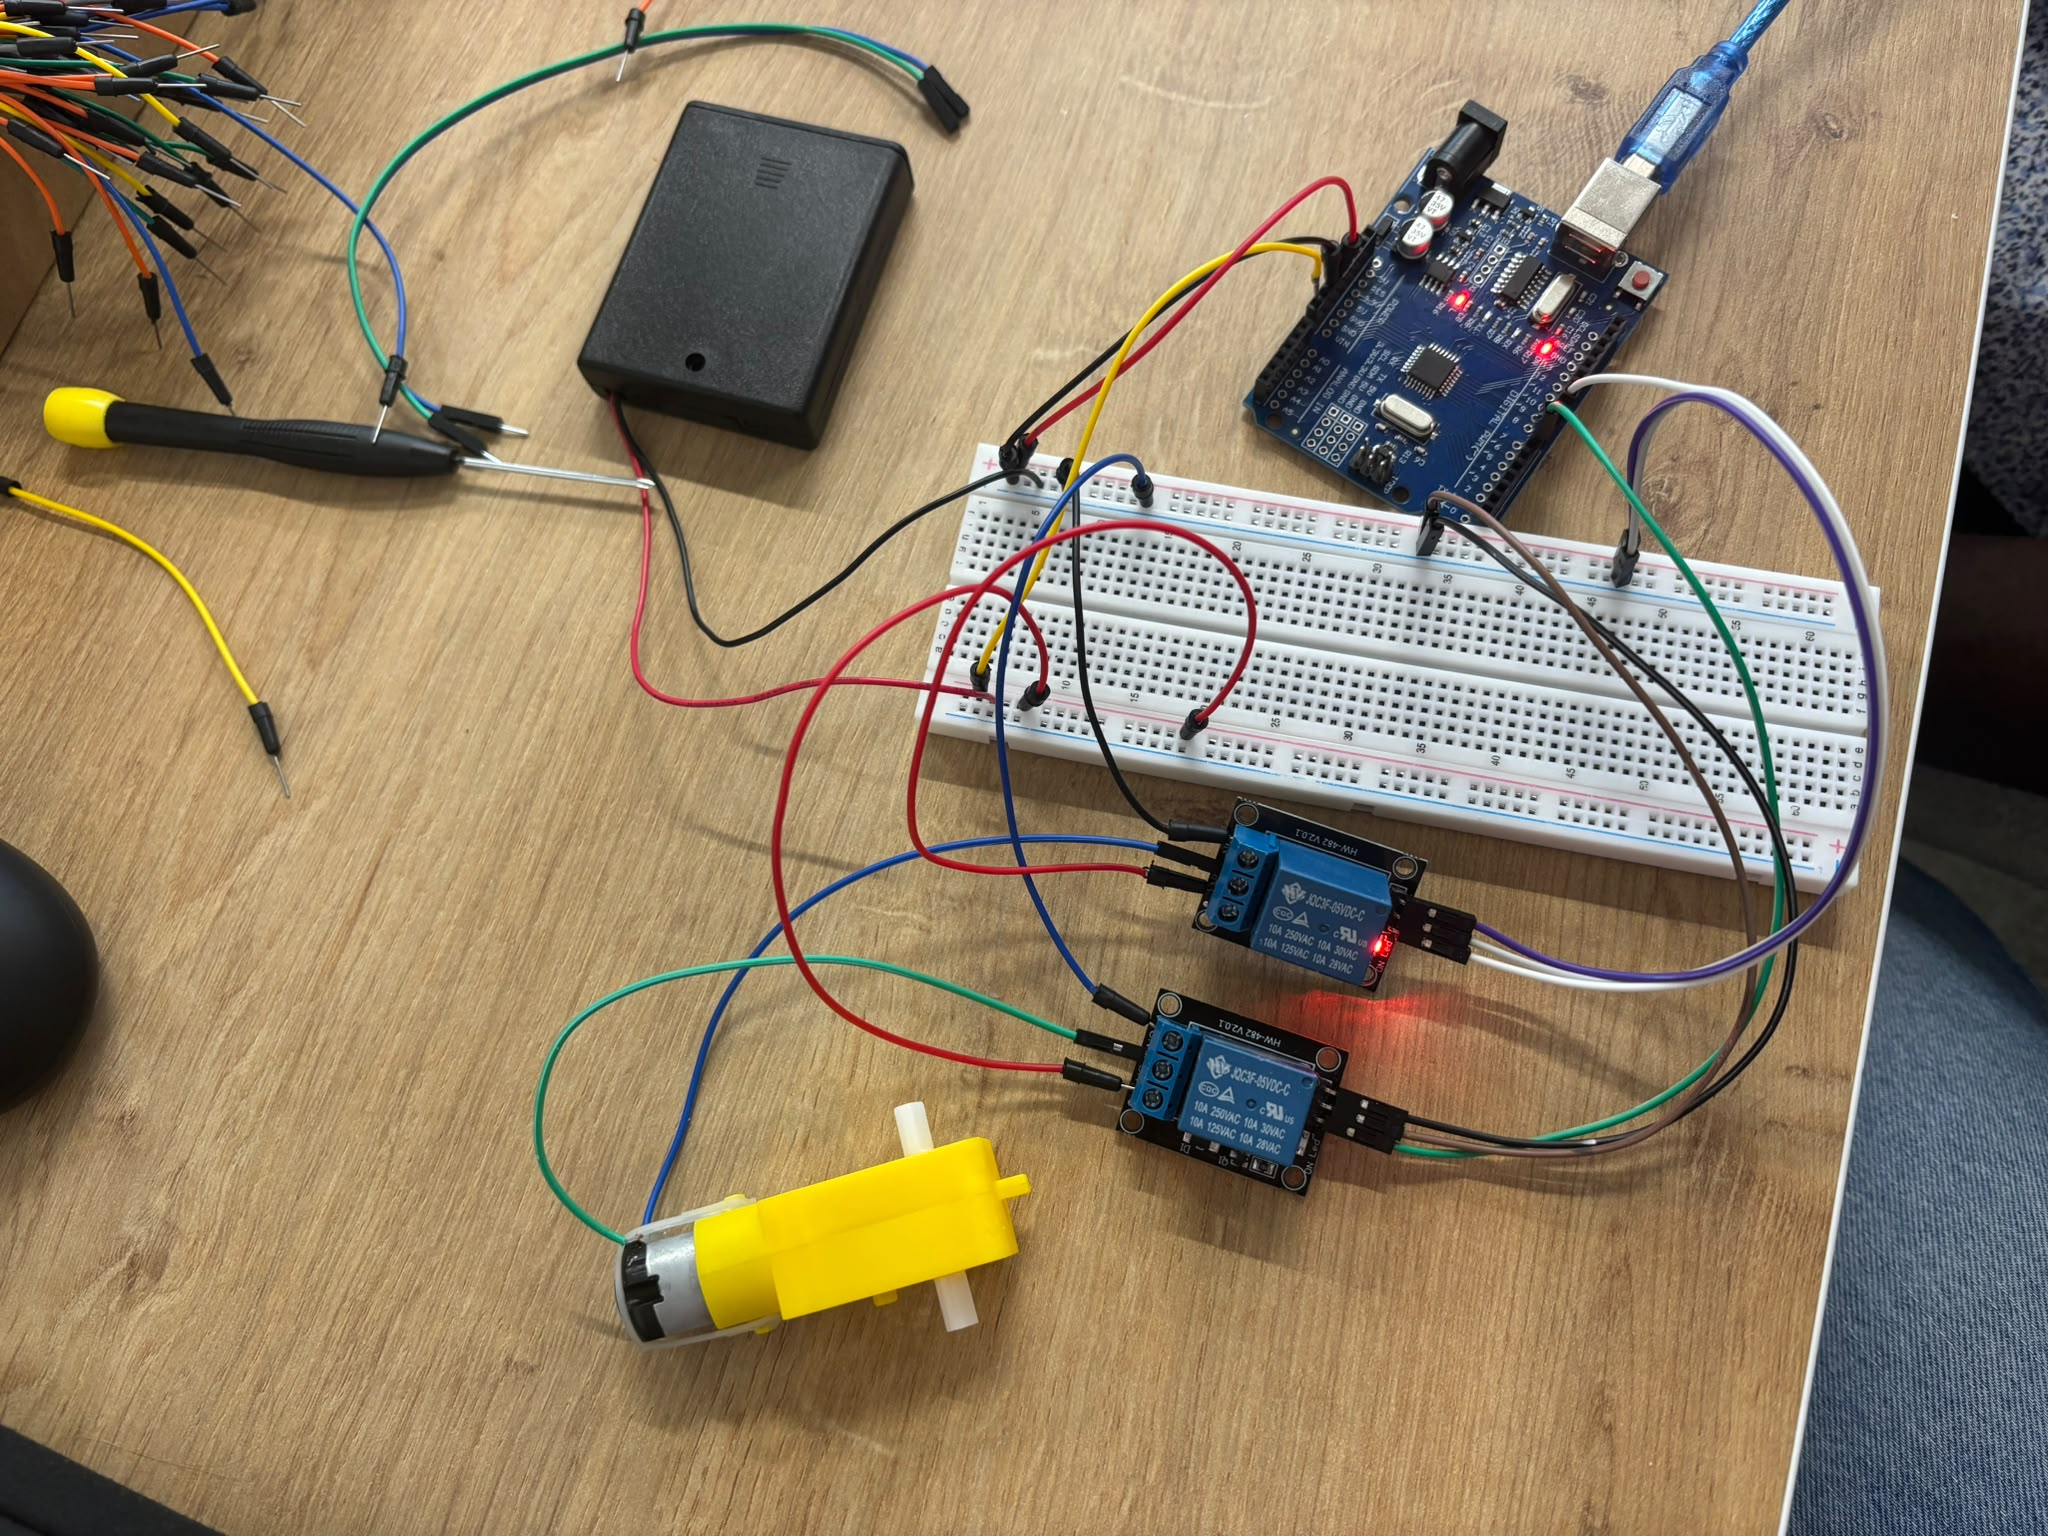
\includegraphics[width=\linewidth]{Image/4.relai}
		\caption{Photo du montage avec relais et moteur DC}
		\label{fig:photo_relais}
	\end{minipage}
\end{figure}

\textbf{Réponses aux questions :}
\begin{enumerate}
	\item \textbf{Comportement du moteur :} Le moteur tourne dans un premier sens pendant 2 secondes, s'arrête 1 seconde, puis tourne dans le sens inverse pendant 2 secondes avant de s'arrêter à nouveau.
	\item \textbf{État des relais :} En observant les LED, on constate que lorsque le Relais 1 est activé (LED allumée) et le Relais 2 au repos, le moteur tourne dans le sens 1. L'inverse produit la rotation dans le sens 2.
	\item \textbf{Phase d'arrêt :} Cette phase est cruciale pour éviter un pic de courant trop important et pour éviter un court circuit.
	\item \textbf{Modification du temps :} Pour modifier les durées, nous avons changé la valeur du premier \texttt{delay()} à \texttt{3000} et celle du second à \texttt{1000}.
\end{enumerate}
\paragraph{Exercice 2 : Commande manuelle par bouton-poussoir}
Nous ajoutons un bouton-poussoir connecté à la broche D9. 
Le programme intègre une gestion de l'anti-rebond (\texttt{debounceDelay} de 50 ms) pour éviter de détecter plusieurs appuis lors d'une seule pression physique.
\begin{figure}[H]
	\centering
	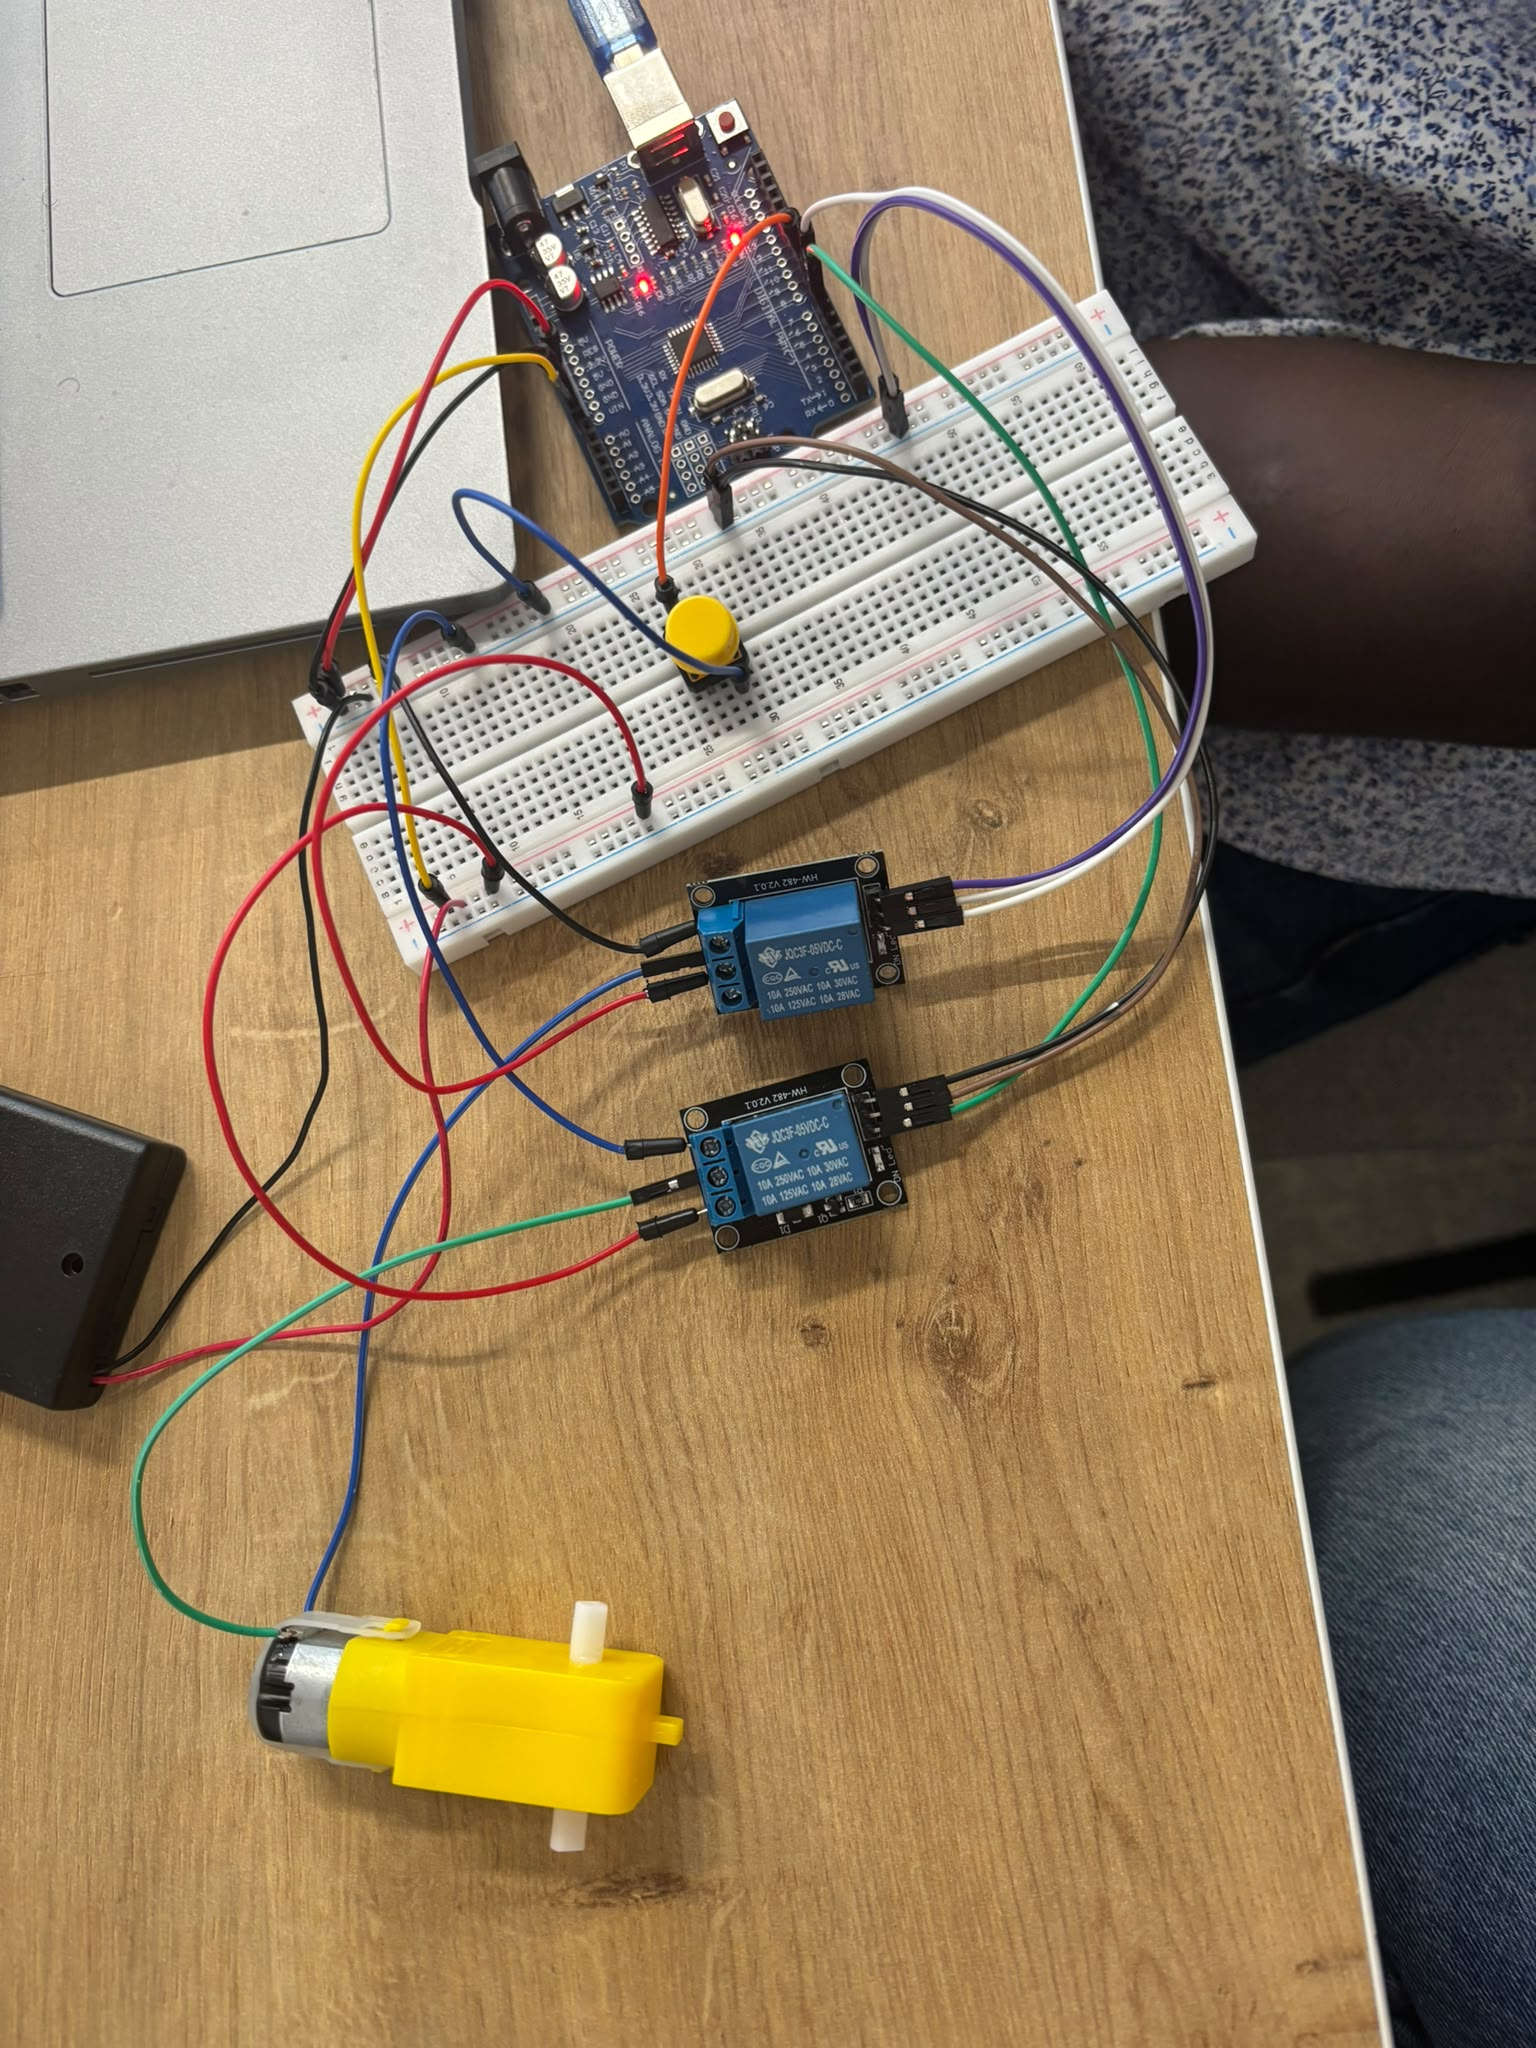
\includegraphics[width=0.5\linewidth]{Image/4.Bouton1}
	\caption{Photo du montage avec 1 bouton-poussoir}
	\label{fig:4}
\end{figure}

\textbf{Réponses aux questions :}
\begin{enumerate}
	\item \textbf{Utilisation de \texttt{INPUT\_PULLUP} :} On utilise la résistance de tirage interne de l'Arduino (activée avec \texttt{INPUT\_PULLUP}) pour simplifier le montage matériel. Cela évite d'avoir à câbler une résistance externe sur la plaque d'essai, tout en fixant un état logique clair (HIGH) lorsque le bouton n'est pas pressé.
	
	\item \textbf{Effet de \texttt{debounceDelay} à 0 :} Si on met la variable \texttt{debounceDelay} à 0, l'anti-rebond  est désactivé. Lors du test, on constate qu'un seul appui physique sur le bouton provoque des changements d'état aléatoires et multiples. Cela est dû aux rebonds mécaniques des contacts du bouton qui sont interprétés comme de multiples appuis successifs.
	
	\item \textbf{Intégration de l'arrêt avant inversion :} La correction a été apportée dans les fonctions de mouvement. Passer d'abord par l'état d'arrêt avec un \texttt{delay(300)} avant d'inverser les relais permet d'éviter les pics de courant, les contraintes mécaniques sur le moteur et l'usure prématurée des contacts des relais, en laissant le temps au moteur de ralentir.
	
	\item \textbf{Ajout d'un second bouton :} Pour utiliser deux boutons (un pour marche/arrêt et un pour le sens de rotation), il faudrait déclarer une seconde entrée avec \texttt{INPUT\_PULLUP} (par exemple sur D10). Le premier bouton basculerait l'état d'une variable booléenne \texttt{moteurActif}, et le second bouton modifierait l'état d'une variable de sens. Les fonctions de commande des relais (\texttt{moveForward} et \texttt{moveReverse}) ne seraient appelées que si \texttt{moteurActif} est vrai.
\end{enumerate}
\begin{figure}[H]
	\centering
	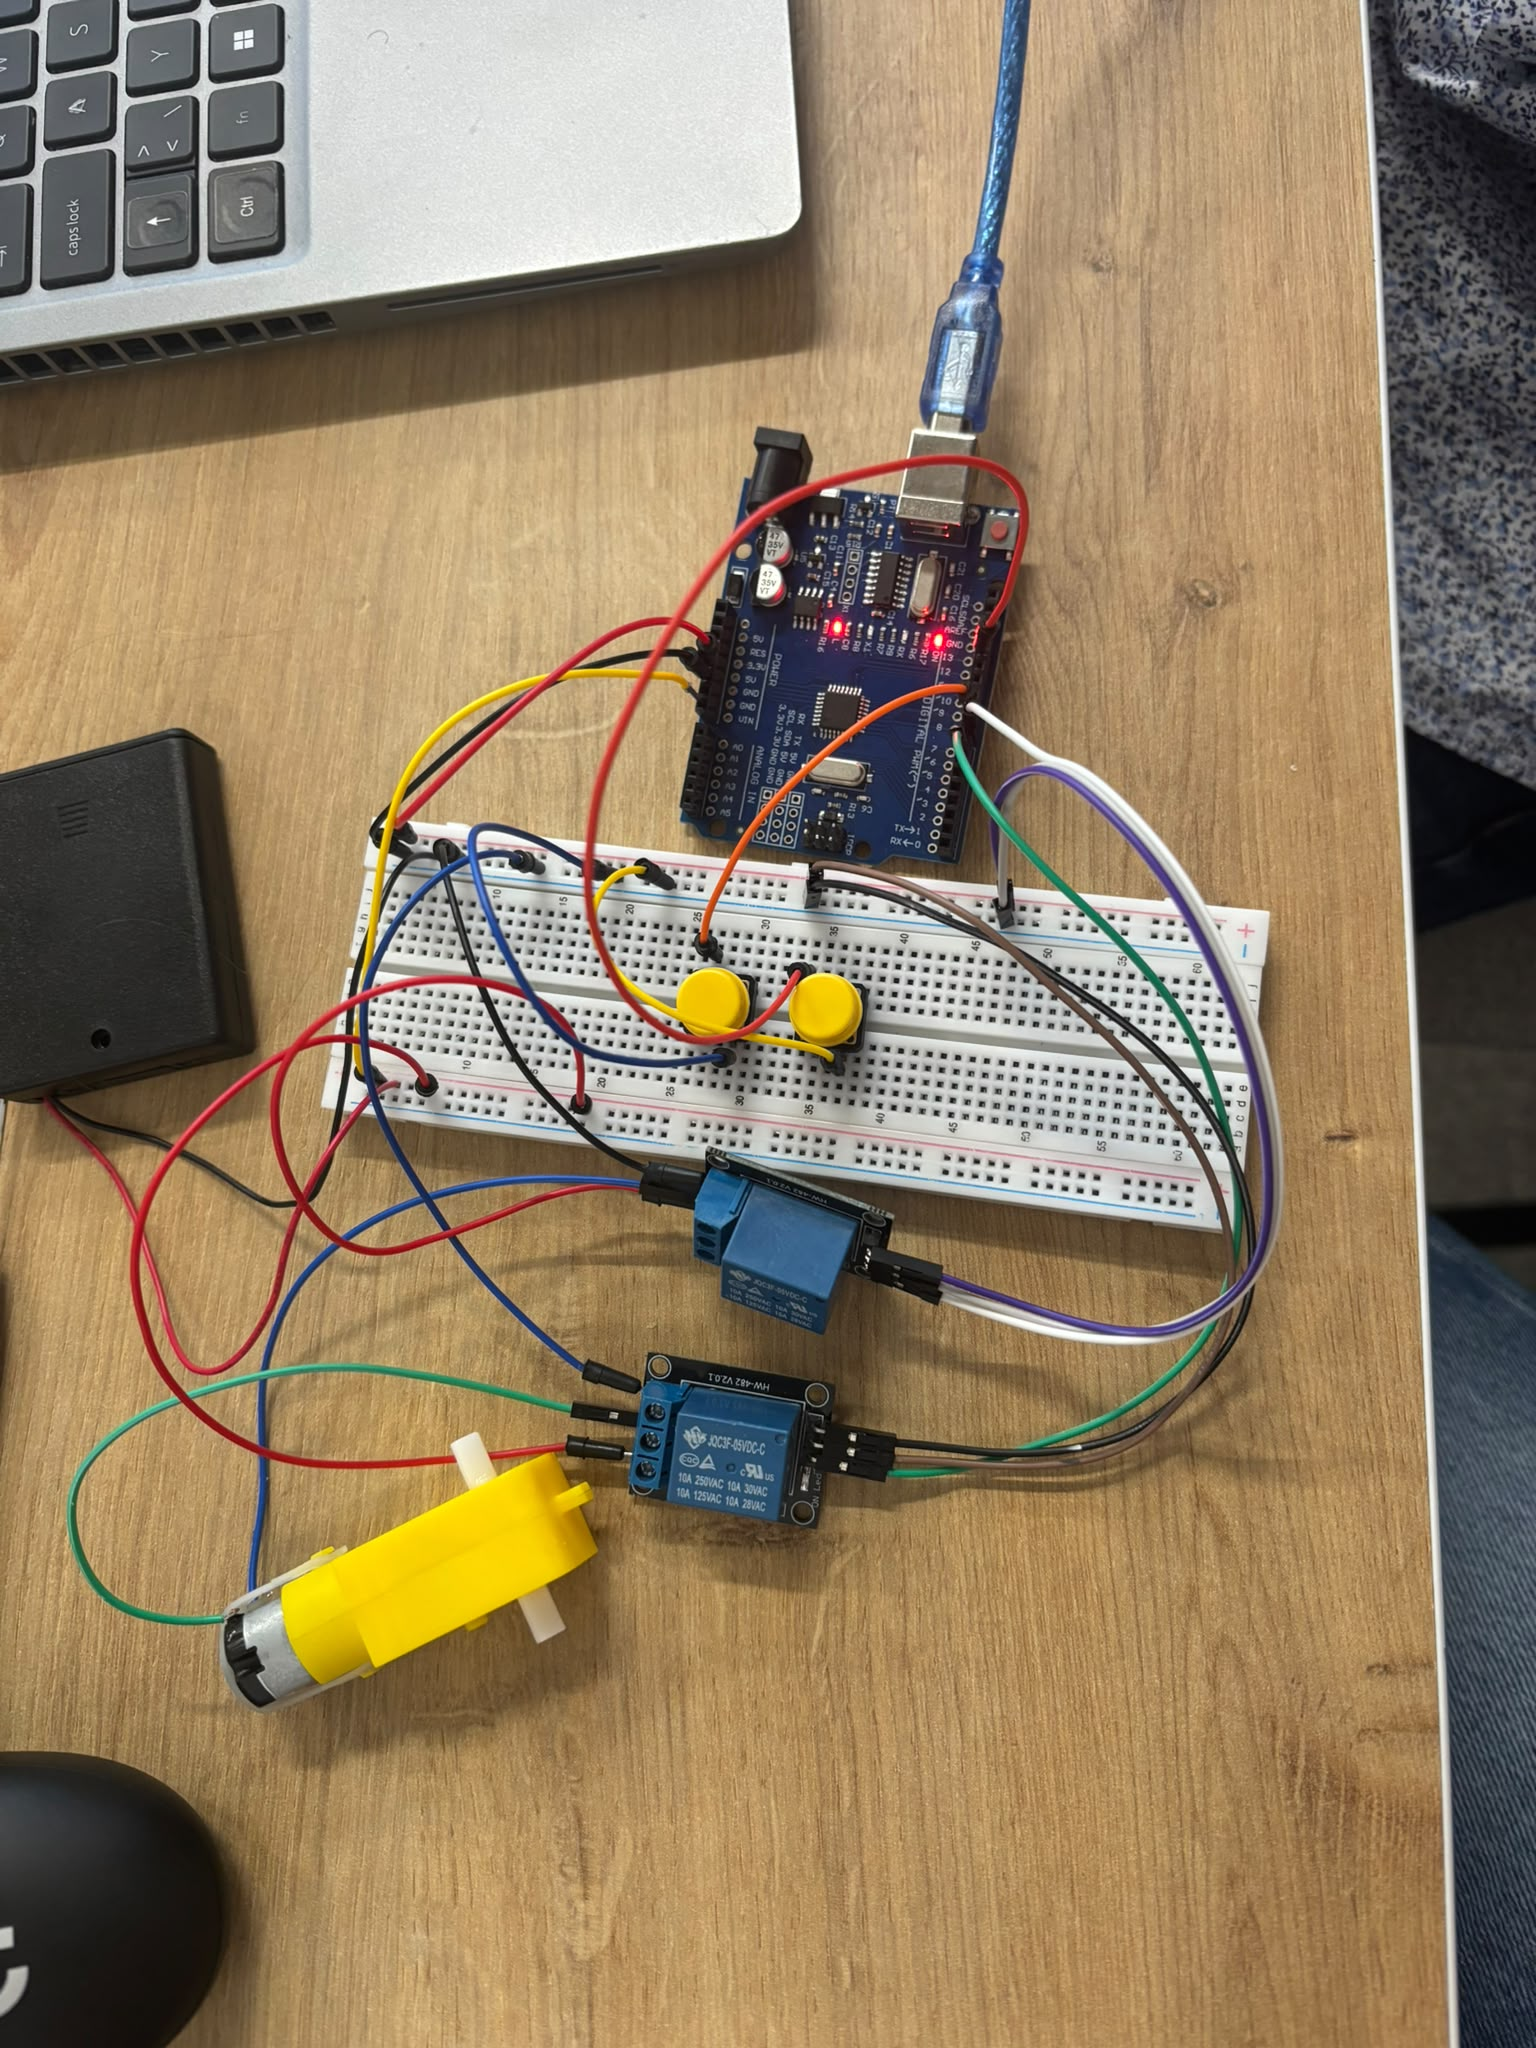
\includegraphics[width=0.5\linewidth]{Image/4.Bouton2}
	\caption{Montage avec deux boutons poussoir}
	\label{fig:4}
\end{figure}

\section{Signal PWM et servomoteur}
La technique PWM (Pulse Width Modulation) permet de simuler une tension analogique en faisant varier le rapport cyclique d'un signal carré. 
Cependant, contrairement à un moteur DC classique, un servomoteur nécessite un signal PWM particulier : des impulsions précises de 1 à 2 ms répétées toutes les 20 ms (50 Hz) pour définir un angle cible. 

\paragraph{Exercice 3 : Positionner un servomoteur à des angles précis}
Nous utilisons la bibliothèque \texttt{Servo.h} au lieu de la commande \texttt{analogWrite()}, car cette dernière ne fonctionne pas à la bonne fréquence. 
Cette bibliothèque permet d'envoyer facilement un angle de consigne (entre 0 et 180 degrés) au servomoteur SG90.

\begin{figure}[H]
	\centering
	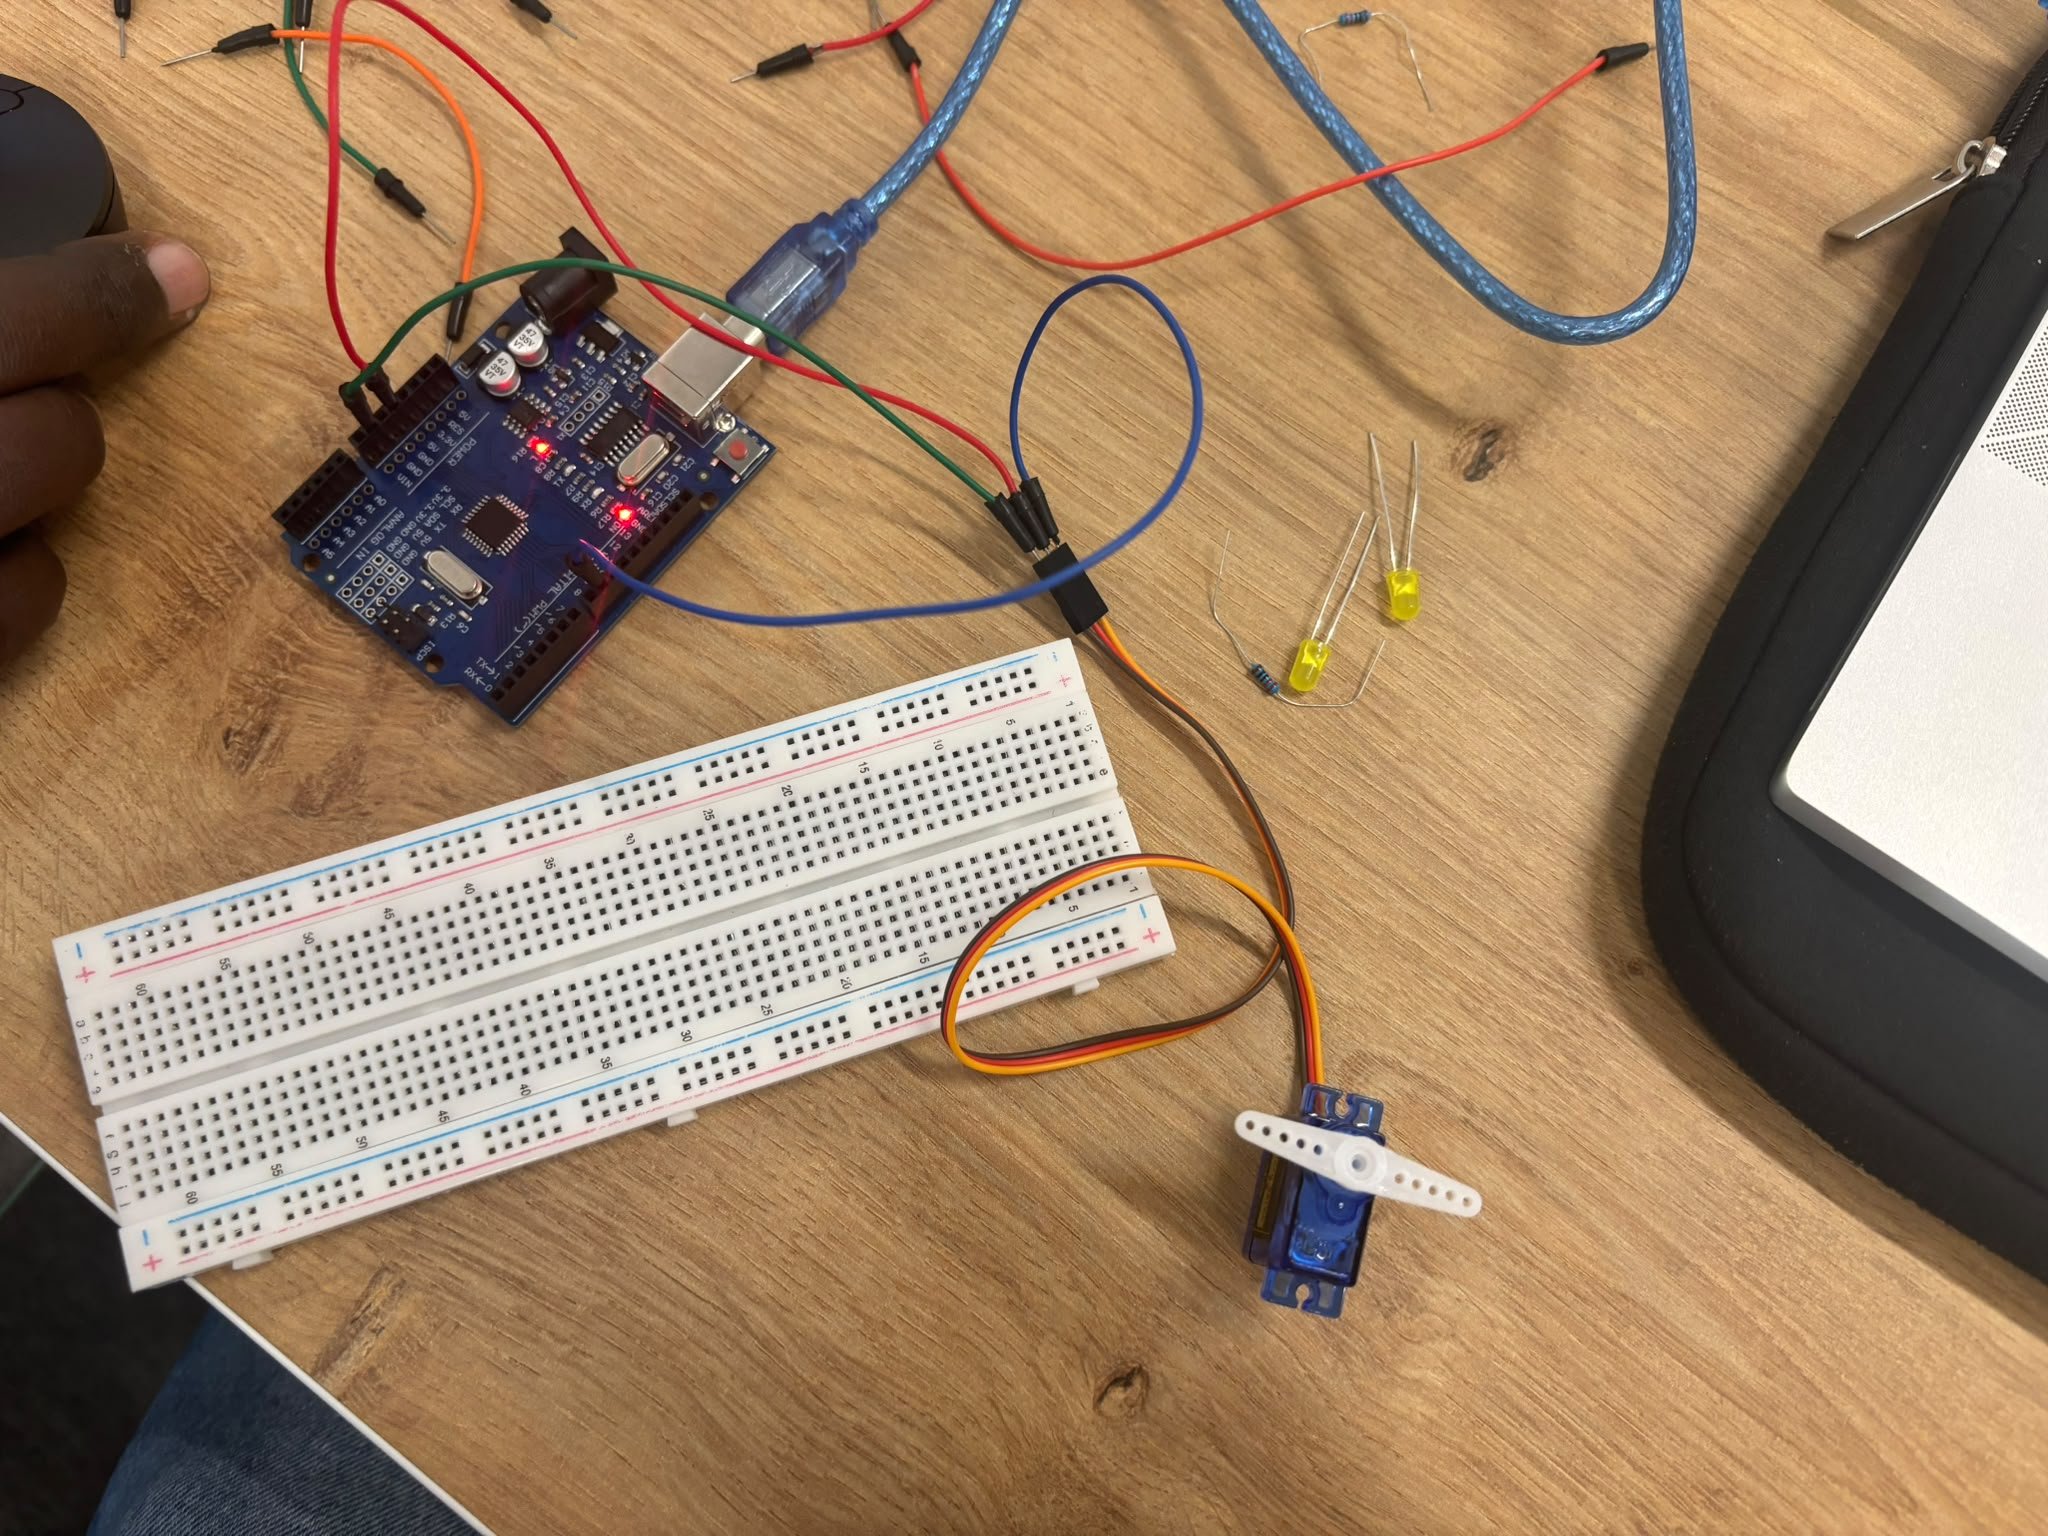
\includegraphics[width=0.7\linewidth]{Image/3.Servo}
	\caption{Servomoteur contrôlé a l'aide de Matlab}
	\label{fig:simulink_led}
\end{figure}

\textbf{Réponses aux questions :}
\begin{enumerate}
	\item \textbf{Différence entre 3-a et 3-b :} Dans le programme 3-a, le mouvement du servomoteur est très saccadé et brutal : il saute directement d'un angle à l'autre (0°, 90°, 180°, 45°) à sa vitesse maximale. Dans le programme 3-b, le mouvement est fluide et progressif (balayage). Le programme décompose le trajet en petits pas de 1° avec un délai de 15 ms entre chaque pas.
	
	\item \textbf{Durée d'un aller (0° $\rightarrow$ 180°) :} Dans le programme 3-b, le balayage s'effectue sur 180 pas (de 0 à 180). Comme le programme attend 15 ms à chaque pas (\texttt{delay(15)}), la durée totale de l'aller est d'environ : $180 \times 15 = 2700\text{ ms}$, soit 2,7 secondes.
	
	\item \textbf{Modification du balayage (aller rapide, retour lent) :} Pour obtenir cet effet, nous avons modifié la première boucle \texttt{for} (aller) en réduisant le délai à \texttt{delay(5)} pour un mouvement rapide, et modifié la seconde boucle \texttt{for} (retour) en augmentant le délai à \texttt{delay(30)} pour un mouvement plus lent.
	
	\begin{lstlisting}
	for (int angle = 180; angle >= 0; angle -= 1) {
		monServo.write(angle);
		delay(5); // ici on change la duree pour changer la vitesse
	}
	delay(1000); // Pause d'une seconde avant de recommencer
	}
		
	\end{lstlisting}
	
	\item \textbf{Précision des butées (0° et 180°) :} Par défaut, les servomoteurs bon marché comme le SG90 n'atteignent pas toujours exactement 0° et 180° avec les valeurs d'impulsions standards (1000 µs à 2000 µs). En utilisant \texttt{monServo.attach(9, 500, 2400)}, on redéfinit les bornes temporelles du signal PWM (500 µs pour 0° et 2400 µs pour 180°). Avec ce réglage, on constate que le servomoteur exploite une plus grande amplitude mécanique et se rapproche beaucoup plus des vraies butées 0° et 180°.
\end{enumerate}

\paragraph{Exercice 4 : Commande du servomoteur par potentiomètre}
Pour piloter manuellement l'angle du servomoteur, nous lisons la tension aux bornes d'un potentiomètre sur l'entrée analogique A0.
La fonction \texttt{map()} nous permet ensuite de convertir cette lecture (de 0 à 1023) en un angle proportionnel compris entre $0^{\circ}$ et $180^{\circ}$.

\begin{figure}[H]
	\centering
	\begin{minipage}{0.48\textwidth}
		\centering
		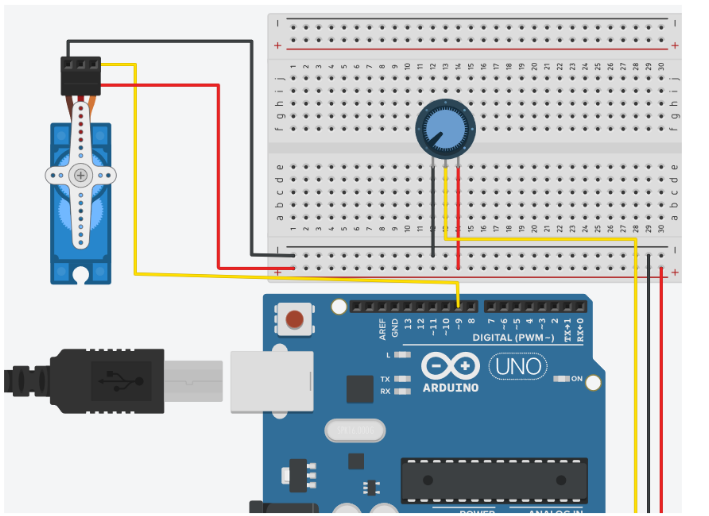
\includegraphics[width=\linewidth]{Image/4.schema_potentiometre}
		\caption{Schéma de la commande par potentiomètre}
		\label{fig:schema_pot_servo}
	\end{minipage}\hfill
	\begin{minipage}{0.48\textwidth}
		\centering
		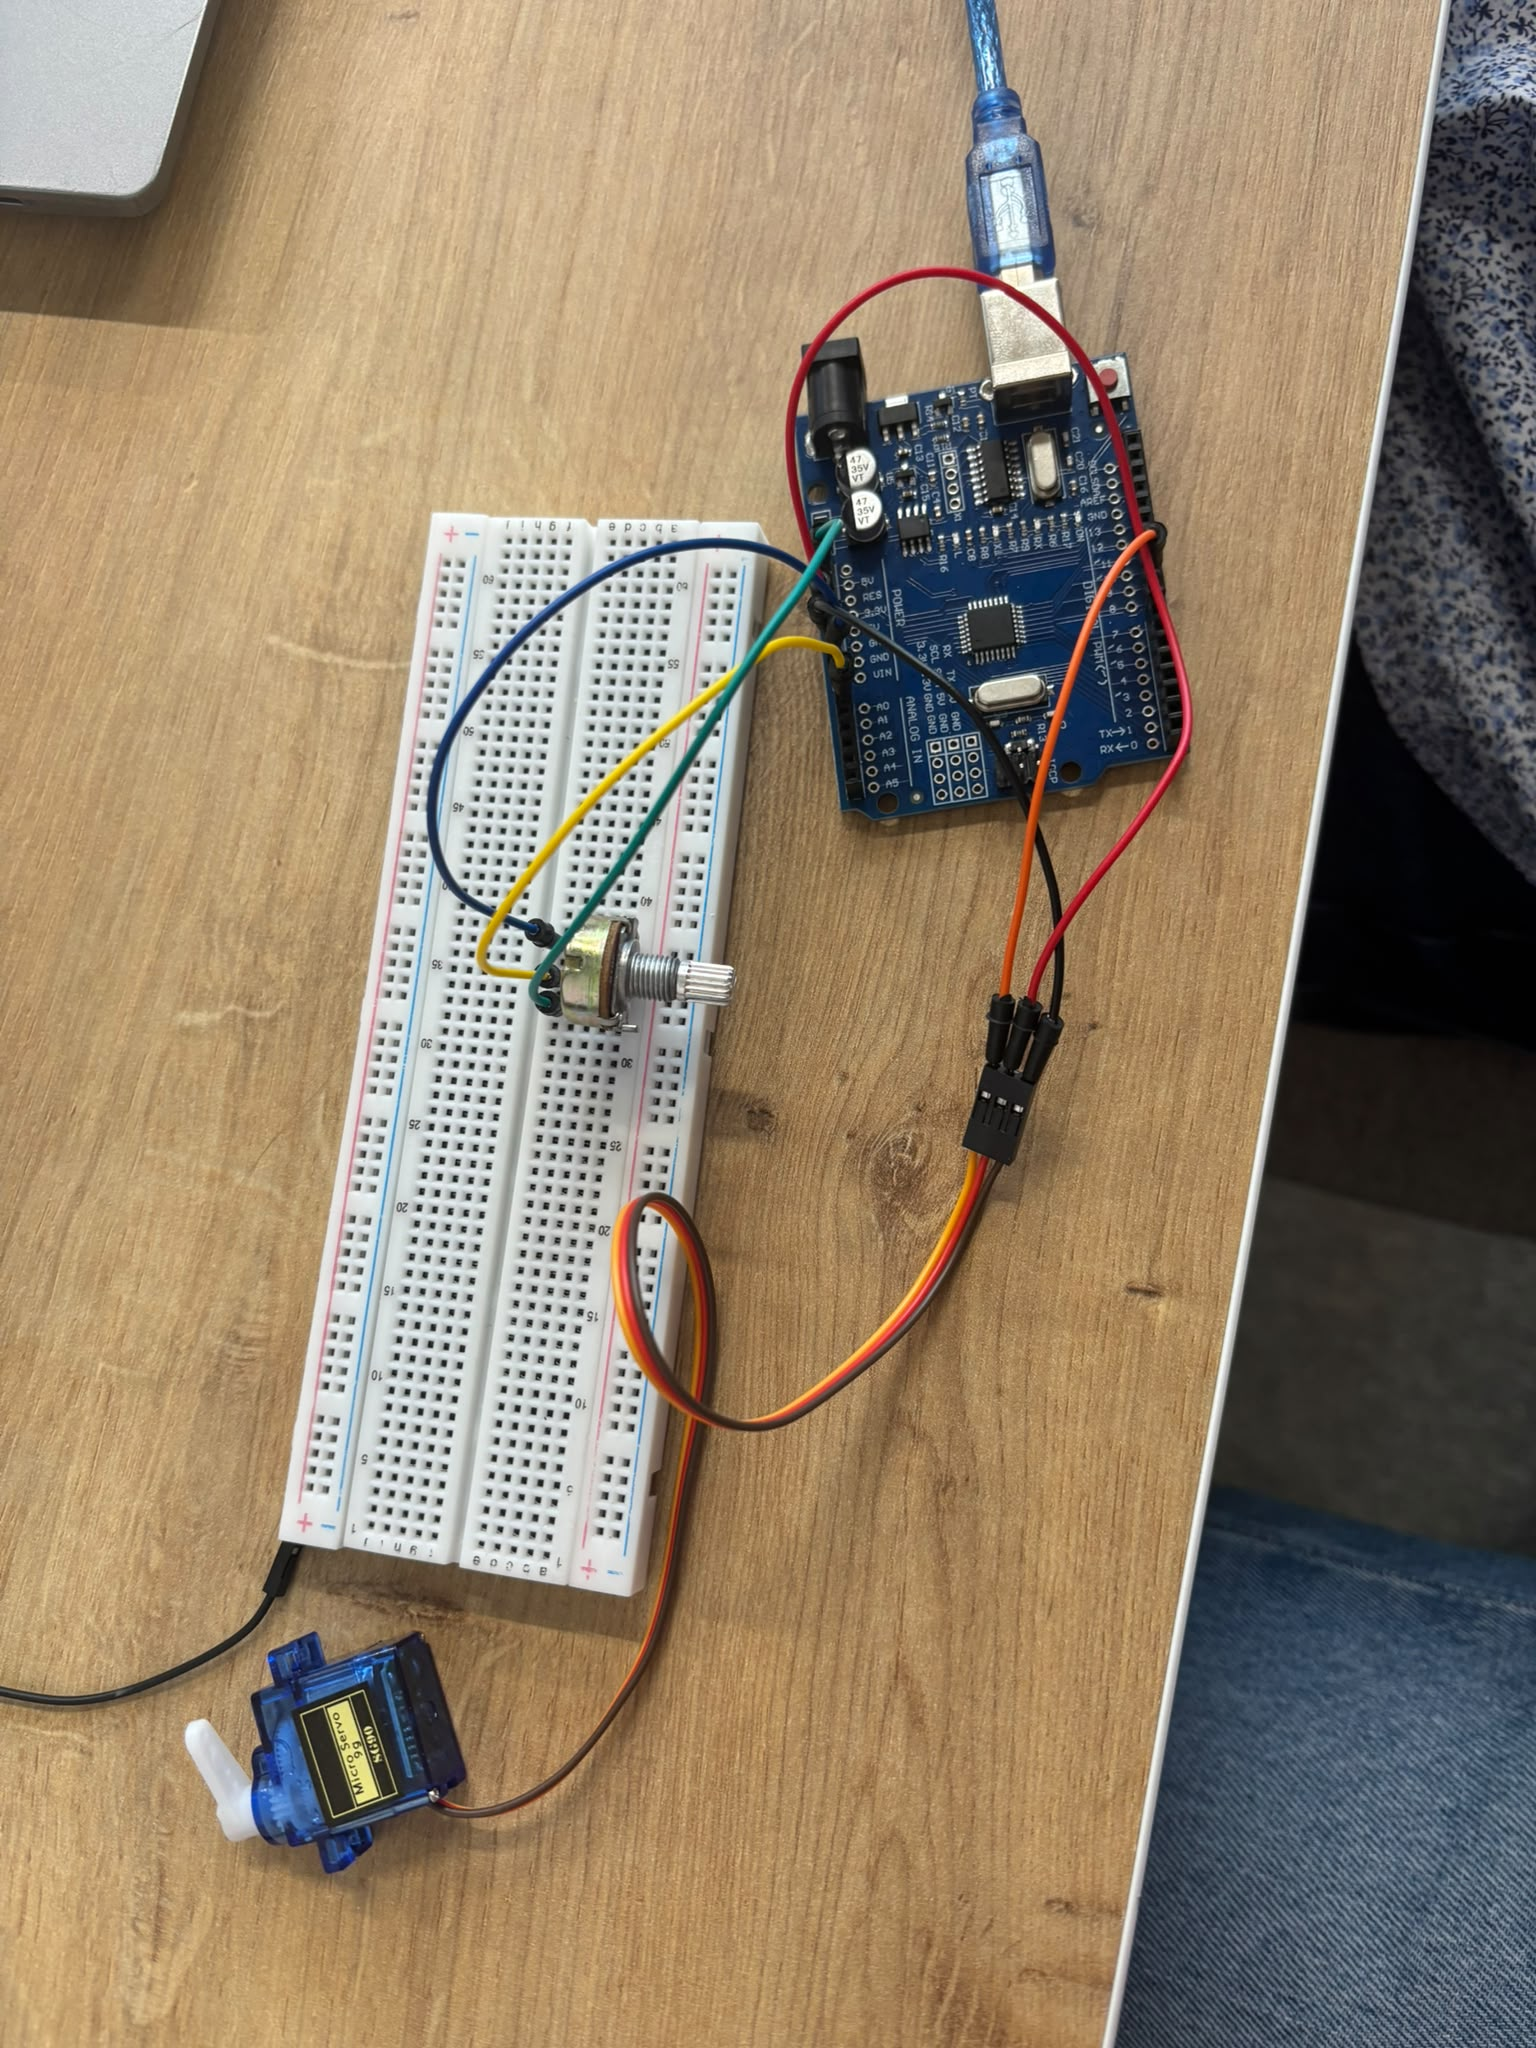
\includegraphics[width=\linewidth]{Image/4.Potentiometre}
		\caption{Photo du montage avec potentiomètre et servomoteur}
		\label{fig:photo_pot_servo}
	\end{minipage}
\end{figure}

\textbf{Réponses aux questions :}
\begin{enumerate}
	\item \textbf{Relevés du moniteur série :} 
	\begin{itemize}
		\item Position 1 : Potentiomètre = 0 $\rightarrow$ Angle = 0°
		\item Position 2 : Potentiomètre = 512 $\rightarrow$ Angle = 90°
		\item Position 3 : Potentiomètre = 1023 $\rightarrow$ Angle = 180°
	\end{itemize}
	
	\item \textbf{Calcul pour la valeur 512 :} La fonction \texttt{map()} réalise un produit en croix (ou interpolation linéaire). La plage du potentiomètre va de 0 à 1023 (amplitude de 1023), et la plage de l'angle va de 0 à 180 (amplitude de 180). Le calcul est : $\text{Angle} = \frac{512 \times 180}{1023} \approx 90,08^\circ$. La valeur affichée est donc bien 90°, ce qui correspond à la position centrale.
	
	\item \textbf{Limitation du mouvement (30° à 150°) :} Pour limiter la plage de mouvement du servomoteur, il suffit de modifier les arguments de sortie de la fonction \texttt{map()} dans le programme. La ligne devient : \texttt{int angle = map(valeurPot, 0, 1023, 30, 150);}. Ainsi, même si le potentiomètre est à 0, le servo n'ira pas en dessous de 30°, et s'il est à 1023, il n'ira pas au-delà de 150°.
	
	\item \textbf{Solution logicielle contre les tremblements :} Pour résoudre cela on enregistre l'ancien angle, et on n'envoie la commande \texttt{monServo.write(angle)} que si la différence absolue entre le nouvel angle calculé et l'ancien est supérieure ou égale à 2°.
	\begin{lstlisting}
	  // 3. Commande du servomoteur avec correction logiciel de l'angle
	int pastAngle = 0 ;
	
	if (abs(newAngle - pastAngle) > 2 ) {
		monServo.write(newAngle);
		pastAngle = newAngle;
	}
	else{
		monServo.write(pastAngle);
	}
	
	\end{lstlisting}
\end{enumerate}